\documentclass[14pt, oneside, a4paper]{extreport}
\usepackage{extsizes}

\usepackage[T1, T2A]{fontenc}
\usepackage[utf8]{inputenc}
\usepackage[english,russian]{babel}
\usepackage{tempora}

\usepackage[left=30mm,right=10mm,top=20mm,bottom=20mm]{geometry}

\usepackage{setspace}
\onehalfspacing

\usepackage{indentfirst}
\setlength{\parindent}{1.25cm}

\usepackage{enumitem}
\setlist{nolistsep}

\renewcommand{\labelitemi}{---}
\renewcommand{\labelenumi}{\arabic{enumi})}

\usepackage{graphicx}
\graphicspath{ {./img/} }

\usepackage{listings}
\lstset{
	basicstyle=\footnotesize\ttfamily,
	numbers=left,
	numberstyle=\tiny,
	numbersep=5pt,
	tabsize=4,
	breaklines=true,
	frame=b,
	stringstyle=\ttfamily\ttfamily,
	showspaces=false,
	showtabs=false,
	xleftmargin=17pt,
	framexleftmargin=17pt,
	framexrightmargin=5pt,
	framexbottommargin=4pt,
	showstringspaces=false,
	inputencoding=utf8x,
	keepspaces=true,
	numberbychapter=false
}

\usepackage{amsmath}
\usepackage{amsfonts}
\usepackage{mathtools}

\usepackage{tikz}
\usepackage{pgfplots}

\usepackage[normalem]{ulem}

\usepackage{titlesec}

\titleformat{\chapter}[block]{\bfseries\normalsize\filcenter}{\thechapter}{1em}{}[
	]
\titlespacing\chapter{\parindent}{-2em}{1em}

\titleformat{\section}[hang]{\bfseries\normalsize}{\thesection}{1em}{}
\titlespacing\section{\parindent}{\parskip}{\parskip}

\titleformat{\subsection}[hang]{\bfseries\normalsize}{\thesubsection}{1em}{}
\titlespacing\subsection{\parindent}{\parskip}{\parskip}

\usepackage{slashbox}

\usepackage{caption}
\captionsetup[figure]{justification=centering}
\DeclareCaptionLabelSeparator{emdash}{\ ---\ }
\captionsetup[figure]{name={Рисунок},labelsep=emdash}
\captionsetup[lstlisting]{justification=raggedright, labelsep=emdash}
\captionsetup[table]{singlelinecheck=false, labelsep=emdash}

\counterwithout{figure}{chapter}
\counterwithout{table}{chapter}
\counterwithout{equation}{chapter}

\newenvironment{sequations} {
\begin{subequations}
\renewcommand{\theequation}{\arabic{parentequation}.\arabic{equation}}
}{
\end{subequations}
}

\usepackage{array}
\newenvironment{signstabular}[1][1]{
	\renewcommand*{\arraystretch}{#1}
	\tabular
}{
	\endtabular
}

\makeatletter
\g@addto@macro\@floatboxreset\centering
\makeatother

\makeatletter
\renewcommand\@biblabel[1]{#1.}
\makeatother

\usepackage{rotating}

\addto\captionsrussian{\renewcommand{\bibname}{Список использованных источников}}

\usepackage{diagbox}

\usepgfplotslibrary{external} 
\tikzexternalize

\usepackage{longtable}
\usepackage{pdfpages}
\usepackage{etoolbox}

\newcounter{totfigures}
\newcounter{tottables}
\newcounter{totpages}
\newcounter{totsources}

\providecommand\totfig{} 
\providecommand\tottab{} 
\providecommand\totpg{}
\providecommand\totsrc{}

\makeatletter
\AtEndDocument{
	\addtocounter{totfigures}{\value{figure}}
	\addtocounter{tottables}{\value{table}}
	\addtocounter{totpages}{\value{page}}
	\addtocounter{totsources}{\value{enumiv}}
	\immediate\write\@mainaux{
	  \string\gdef\string\totfig{\number\value{totfigures}}
	  \string\gdef\string\tottab{\number\value{tottables}}
	  \string\gdef\string\totpg{\number\value{totpages}}
	  \string\gdef\string\totsrc{\number\value{totsources}}
	}
}
\makeatother

\addto\captionsrussian{% Replace "english" with the language you use
  \renewcommand{\contentsname}%
    {Содержание}%
}


\begin{document}

\begin{titlepage}
	\noindent\begin{minipage}{0.05\textwidth}
		
\includegraphics[scale=0.3]{bmstu.png}
	\end{minipage}
	\hfill
	\begin{minipage}{0.85\textwidth}\raggedleft
		\begin{center}
			\fontsize{12pt}{0.3\baselineskip}\selectfont \textbf{Министерство науки и высшего образования Российской Федерации \\ Федеральное государственное бюджетное образовательное учреждение \\ высшего образования \\ <<Московский государственный технический университет \\ имени Н.Э. Баумана \\ (национальный исследовательский университет)>> \\ (МГТУ им. Н.Э. Баумана)}
		\end{center}
	\end{minipage}
	
	\begin{center}
		\fontsize{12pt}{0.1\baselineskip}\selectfont
		\noindent\makebox[\linewidth]{\rule{\textwidth}{4pt}} \makebox[\linewidth]{\rule{\textwidth}{1pt}}
	\end{center}
	
	\begin{flushleft}
		\fontsize{12pt}{0.8\baselineskip}\selectfont 
		
		ФАКУЛЬТЕТ \uline{<<\textbf{Информатика и системы управления}>> \hfill}
		
		КАФЕДРА \uline{<<\textbf{Программное обеспечение ЭВМ и информационные технологии}>> \hfill}
		
		ДИСЦИПЛИНА \uline{<<\textbf{Защита информации}>> \hfill}
	\end{flushleft}
	
	\vfill
	
	\begin{center}
		\fontsize{18pt}{\baselineskip}\selectfont
		
		\textbf{ОТЧЁТ}
		
		\textbf{\textit{К ЛАБОРАТОРНОЙ РАБОТЕ 1}}
		
		\textbf{\textit{НА ТЕМУ:}}
	\end{center}
	
	\begin{center}
		\fontsize{18pt}{0.6cm}\selectfont 
		
		<<Энигма>>
		
	\end{center}
	
	\vfill
	
	\begin{table}[h!]
		\fontsize{12pt}{0.7\baselineskip}\selectfont
		\centering
		\begin{signstabular}[0.7]{p{7.25cm} >{\centering\arraybackslash}p{4cm} >{\centering\arraybackslash}p{4cm}}
			Студент группы \textbf{ИУ7-72Б} & \uline{\mbox{\hspace*{4cm}}} & \uline{\hfill \textbf{Комаров Н.С.} \hfill} \\
			& \scriptsize (Подпись, дата) & \scriptsize (Фамилия И.О.)
		\end{signstabular}
		
		\vspace{\baselineskip}
		
		\begin{signstabular}[0.7]{p{7.25cm} >{\centering\arraybackslash}p{4cm} >{\centering\arraybackslash}p{4cm}}
			Преподаватель & \uline{\mbox{\hspace*{4cm}}} & \uline{\hfill \textbf{Чиж И.С.} \hfill} \\
			& \scriptsize (Подпись, дата) & \scriptsize (Фамилия И.О.)
		\end{signstabular}
	\end{table}
	
	\vfill
	
	\begin{center}
		\normalsize \textbf{2023} г.
	\end{center}
\end{titlepage}

\setcounter{page}{2}

\chapter{<<Энигма>>}
<<Энигма>> состоит из трёх основных элементов: коммутационная панель, набор роторов и рефлектор. На машине присутствует клавиатура со всеми буквами алфавита. По нажатии на любую клавишу, проворачиваются роторы. Сигнал проходит сначала через коммутационную панель, потом через все роторы, и затем приходит в рефлектор, отражающий сигнал обратно через роторы, но уже в обратном направлении. В последний раз пройдя через коммутационную панель, электрический сигнал подсвечивает одну из лампочек, обозначенные буквами алфавита.

\section{Коммутационная панель}
Коммутационная панель представляет собой набор гнёзд под каждую букву алфавита. В комплекте с <<Энигмой>> идёт набор проводов, позволяющий соединить любую пару таких <<слотов>> между собой.

Коммутационная панель выполняет подмену одного символа на другой для сигнала идущего на вход, и для другого сигнала, идущего на выход. По сути, является биекцией одного подмножества алфавита в другое не пересекающееся с первым.

\section{Роторы}
Роторы представляют собой диски, с наборами контактов с обеих сторон. Контакты одной стороны произвольным образом связаны с контактами другой. При нажатии на клавишу, происходит поворот последнего диска. Когда любой из роторов совершает полный оборот (переводящий его на значение 1), проворачивается диск слева от него. Каждый диск, по сути, является биекцией алфавита на самого себя.

\section{Рефлектор}
Рефлектор --- компонент <<Энигмы>>, отличающий её от других роторных машин. По логике работы ничем не отличается от коммутационной панели, отличие только в том, что работает не на вводе/выводе, а между прямым и обратным ходом сигнала

\chapter{Разработка программы}
Программа была реализована на языке <<C++>> без использования каких-либо дополнительных сторонних библиотек. Количество роторов --- 3, но может быть изменено при перекомпиляции. Начальная конфигурация роторов (их поворот) точно также может быть изменена.

\section{Архитектура}
При реализации программы были выделены классы для каждого из компонентов <<Энигмы>>. UML диаграмма представлена на рис. \ref{fig:uml}. Класс <<Permutator>> хранит в себе строку перестановки, позволяющую отображать алфавит на самого себя, и предоставляет методы для выполнения этой перестановки в обе стороны. Остальные классы, используя <<Permutator>>, выполняют каждый свою логику обработки символа: ротор использует биекцию алфавита на самого себя, смещая буквы в зависимости от значения поворота; рефлектор и коммутационная панель используют только биекцию двух половин алфавита.

\begin{figure}[!ht]
    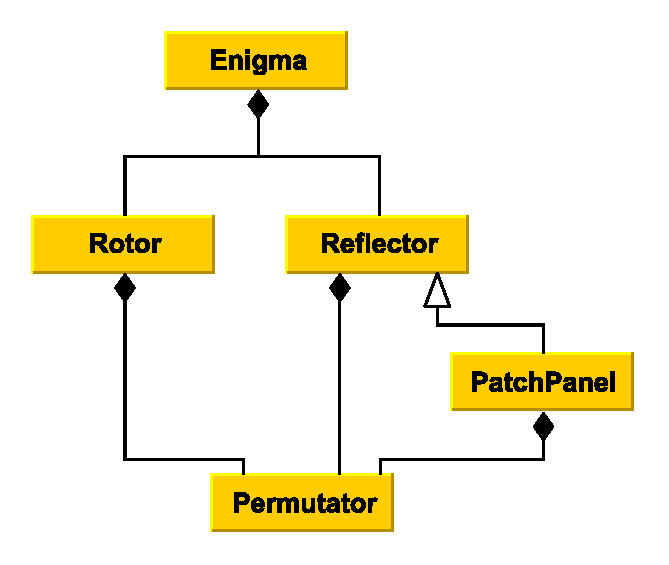
\includegraphics[width=0.4\linewidth]{uml}
    \caption{UML диаграмма программы}
    \label{fig:uml}
\end{figure}

\section{Режимы работы}
Программа может быть собрана для трёх вариантов работы:
\begin{enumerate}
    \item в файлах кодировки Windows1251 заменять только буквы русского алфавита;
    \item в файлах кодировки Windows1251 заменять только буквы английского алфавита;
    \item в любых бинарных файлах работать со всеми байтами (алфавит объёма 256 символов).
\end{enumerate}

\section{Ввод/вывод}
Программа работает с файлами. Чтобы зашифровать файл, необходимо его указать первым и единственным параметром при запуске программы. Если параметр не указан или их неверное число, программа примет название файла "input". Если файл не будет найден, сообщение об этом будет выведено в stdout.

Программа так-же выводит в stdout подробный путь каждого символа, в случае если программа не работает в режиме обработки бинарных файлов.

\section{Пример работы программы}
Текст входного файла в кодировке cp1251 и с CRLF переносами строк представлен на листинге \ref{lst:in}.
\begin{lstlisting}[caption={Входной файл}, label={lst:in}]
Hello, world! aaaa
Hello, world!
\end{lstlisting}

Создаваемый программой выходной файл при работе в режиме обработки английского текста представлен на листинге \ref{lst:out-eng}.
\begin{lstlisting}[caption={Входной файл}, label={lst:out-eng}]
MGDZT, URFGJ! FYVD
AYYBY, QIYOE!
\end{lstlisting}

На листинге \ref{lst:out-eng-stdout} представлен сокращённый вывод программы в stdin.

\begin{lstlisting}[caption={Вывод в stdout для первых трёх букв}, label={lst:out-eng-stdout}]
H >|K|> R >|P|> O >|P|> Y >|P|> X >|
   |O|     |T|     |T|     |T|     |REFLECTOR
M <|M|< N <|1|< G <|2|< J <|3|< J <| 

e >|K|> W >|P|> Y >|P|> Z >|P|> S >|
   |O|     |T|     |T|     |T|     |REFLECTOR
G <|M|< V <|1|< E <|2|< B <|3|< F <|

l >|K|> U >|P|> W >|P|> Q >|P|> B >|
   |O|     |T|     |T|     |T|     |REFLECTOR
D <|M|< Y <|1|< X <|2|< I <|3|< Y <|
\end{lstlisting}

Содержимое файла, полученное в результате прогона выходного файла через программу с той же конфигурацией, отличается от представленного на листинге \ref{lst:in} только тем, что все английские буквы имеют верхний регистр.

\chapter{Тестирование}
Тестирование нужно производить для каждого отдельного компонента <<Энигмы>>, и для всей программы в целом.

\section{Чёрный ящик}
Для режима работы с буквенным алфавитом, тестирование всей программы проведено с помощью файла, в котором по нескольку раз перечислены все буквы алфавита в том же самом порядке, и затем в последующем прогоне программы через тот же файл в той же самой конфигурации машины. Если повторный прогон совпадает с исходным файлом, значит программа работает исправно. Важно убедиться в том, что зашифрованный файл обладает свойствами присущими результату шифрования энигме: две одинаковые буквы могут быть зашифрованы разными символами, а два разных символа могут быть зашифрованы одним. При этом, никакой из символов исходного файла не будет соответствовать самому себе в итоговом.

Пример содержимого файла для такого тестирования приведён на листинге \ref{lst:test}.
\begin{lstlisting}[caption={Содержимое файла для тестирования программы в режиме работы с алфавитом}, label={lst:test}]
ABCDEFGHIJKLMNOPQRSTUVWXYZ
abcdefghijklmnopqrstuvwxyz
,.]\]'['
aaaa AAAA bbbb BBBB
\end{lstlisting}

Для тестирования бинарного режима работы, можно применить похожий метод, но в качестве входного файла использовать несколько последовательностей байт от 0 до 255 включительно.

\section{Белый ящик}
Чтобы убедиться, что программа работает также как <<Энигма>>, необходимо проверить корректность работы каждого из её отдельных компонентов.

\subsection{Коммутационная панель и рефлектор}
Коммутационная панель и рефлектор работают по одному принципу, поэтому их тестирование производится аналогичным образом.

При прогоне через этот компонент любую половину алфавита, на выходе должна получиться полностью отличающаяся часть, и при повторном прогоне полученного результата, должен получиться изначальный ввод.

Даже при прогоне полного алфавита, в результате не должно оказаться повторений.

\subsection{Роторы}
Для роторов, важно протестировать то, что они правильно выполняют оборот, и что правильно отображают букву, причём в обе стороны.

Первое можно проверить, задав ротору в качестве биекции прямой алфавит. Тогда можно легко увидеть, какой именно сдвиг у ротора на текущий момент просто по его выводу. Здесь нужно проверить работу роторов при нулевом изначальном обороте, и при последнем --- чтобы убедиться в том, что каждый ротор поворачивает за собой другой при полном обороте.

Помимо этого, необходимо проверить то, что роторы работают в обе стороны. По сути, нужно убедиться, что отображение левой и правой части диска является биекцией. Для этого, с выключенным проворотом, для каждой буквы выполняем прямой проход по одному ротору, а результат отправляем в обратный ход. После такой манипуляции, итоговая буква должна совпадать с начальной.

%\tableofcontents

%\addcontentsline{toc}{chapter}{Список использованных источников}
%\bibliographystyle{utf8gost705u}
%\bibliography{sources}

\end{document}
